\documentclass[]{elsarticle} %review=doublespace preprint=single 5p=2 column
%%% Begin My package additions %%%%%%%%%%%%%%%%%%%
\usepackage[hyphens]{url}

  \journal{Transportation Research Part D: Transport and Environment} % Sets Journal name


\usepackage{lineno} % add
\providecommand{\tightlist}{%
  \setlength{\itemsep}{0pt}\setlength{\parskip}{0pt}}

\usepackage{graphicx}
\usepackage{booktabs} % book-quality tables
%%%%%%%%%%%%%%%% end my additions to header

\usepackage[T1]{fontenc}
\usepackage{lmodern}
\usepackage{amssymb,amsmath}
\usepackage{ifxetex,ifluatex}
\usepackage{fixltx2e} % provides \textsubscript
% use upquote if available, for straight quotes in verbatim environments
\IfFileExists{upquote.sty}{\usepackage{upquote}}{}
\ifnum 0\ifxetex 1\fi\ifluatex 1\fi=0 % if pdftex
  \usepackage[utf8]{inputenc}
\else % if luatex or xelatex
  \usepackage{fontspec}
  \ifxetex
    \usepackage{xltxtra,xunicode}
  \fi
  \defaultfontfeatures{Mapping=tex-text,Scale=MatchLowercase}
  \newcommand{\euro}{€}
\fi
% use microtype if available
\IfFileExists{microtype.sty}{\usepackage{microtype}}{}
\bibliographystyle{elsarticle-harv}
\ifxetex
  \usepackage[setpagesize=false, % page size defined by xetex
              unicode=false, % unicode breaks when used with xetex
              xetex]{hyperref}
\else
  \usepackage[unicode=true]{hyperref}
\fi
\hypersetup{breaklinks=true,
            bookmarks=true,
            pdfauthor={},
            pdftitle={Examining spatial equity and accessibility to a public bicycle share program using a balanced floating catchment area approach},
            colorlinks=false,
            urlcolor=blue,
            linkcolor=magenta,
            pdfborder={0 0 0}}
\urlstyle{same}  % don't use monospace font for urls

\setcounter{secnumdepth}{0}
% Pandoc toggle for numbering sections (defaults to be off)
\setcounter{secnumdepth}{0}

% Pandoc citation processing

% Pandoc header
\usepackage{booktabs}
\usepackage{longtable}
\usepackage{array}
\usepackage{multirow}
\usepackage{wrapfig}
\usepackage{float}
\usepackage{colortbl}
\usepackage{pdflscape}
\usepackage{tabu}
\usepackage{threeparttable}
\usepackage{threeparttablex}
\usepackage[normalem]{ulem}
\usepackage{makecell}
\usepackage{xcolor}



\begin{document}
\begin{frontmatter}

  \title{Examining spatial equity and accessibility to a public bicycle share
program using a balanced floating catchment area approach}
    \author[Some School]{Elise Desjardins\corref{1}}
   \ead{desjae@mcmaster.ca} 
    \author[Another University]{Christopher D. Higgins\corref{2}}
   \ead{cd.higgins@utoronto.ca} 
    \author[Some School]{Antonio Paez\corref{2}}
   \ead{paezha@mcmaster.ca} 
      \address[McMaster University]{School of Earth, Environment \& Society, 1280 Main Street West,
Hamilton, ON L8S4L8}
    \address[University of Toronto Scarborough]{Department of Geography \& Planning, 1265 Military Trail, Toronto, ON
M1C1A4}
      \cortext[1]{Corresponding Author}
    \cortext[2]{Equal contribution}
  
  \begin{abstract}
  Public bicycle share programs are implemented to promote cycling as a
  convenient and sustainable mode of transportation. These systems can
  also play a role in addressing transportation needs and advancing
  transportation equity if they make cycling more accessible to lower
  income or disadvantaged populations. Recent studies assessing equity in
  bike sharing have found differences in ridership or membership based on
  income, education, and trip purpose. In Ontario, the City of Hamilton
  launched a public bicycle share program in 2015 that currently has over
  900 operational bicycles and 130 docking stations. In 2018, the
  non-profit organization that operates the program launched an equity
  initiative to provide subsidized memberships and to expand service by
  adding twelve docking stations. Previous research found that Hamilton's
  public bicycle share program targeted well disadvantaged areas in the
  city compared to programs in other Canadian cities. Since the time or
  distance that members of the population need to reach a bicycle share
  station decreases the potential of accessing the program, the location
  of stations matters. Unlike other public amenities with greater ability
  to adapt to crowding, the utility of stations is limited by the number
  of bicycles that they can hold, which makes crowding effects critical;
  the system may not necessarily be improved if stations are easy to reach
  but offer only a small number of bicycles. In this research, we revisit
  the case of Hamilton and investigate equity differentials in
  accessibility to bicycle share stations. We compare accessibility in the
  program with and without the equity stations to assess the effect of the
  initiative. Previous research on cycling equity or accessibility has
  used a macro-level approach with entire neighbourhoods or census tracts
  as the unit of analysis, although there are recent exceptions. In
  contrast, we implement our analysis parting from microscopic zones to
  better reflect travel to a docking station, which often happens at the
  sub-neighborhood level, and conduct a sensitivity analysis at several
  walking thresholds. We then reaggregate the estimated accessibility to
  dissemination areas for further analysis using census data. Equity
  analysis of this type is possible thanks to a newly developed approach
  for accessibility using balanced floating catchment areas. The addition
  of equity stations achieved its goal to increase accessibility for lower
  income populations, although the increase was relatively modest (2.10
  bicycles/person with equity stations vs 1.97 bicycles/person without
  equity stations). Further research is needed to determine whether this
  encouraged more cycling.
  \end{abstract}
  
 \end{frontmatter}

\hypertarget{background}{%
\section{Background}\label{background}}

Public bicycle share programs (PBSP) have been implemented in over 800
cities worldwide and a great deal has been learned about their typical
users (Fishman, 2016). In many cities, males use bike share more than
females (Brey et al., 2017; Nickkar et al., 2019; Reilly, S. M. Wang, et
al., 2020; Winters et al., 2019) as do younger age cohorts (Brey et al.,
2017; Buck et al., 2013; Fuller et al., 2011). However, one study found
that bike share users in Washington, DC were more likely to be female
(Buck et al., 2013), which suggests that the gender gap among cyclists
who use bike share is less disparate than the gap for personal bicycle
use (Fishman, 2016). There is some evidence that bike share users are
less likely to own a car (Buck et al., 2013; Reilly, Noyes, et al.,
2020). However, the relationship between income or education and bike
share use is less clear. Stations in disadvantaged communities in
Chicago generated most of the average annual trips (Qian and Jaller,
2020) and individuals from minority or lower socioeconomic status
neighbourhoods in Minneapolis-St.~Paul used the city's PBSP more (J.
Wang and Lindsey, 2019a). Being university educated was also a
significant correlate of bike share use in Montreal, Canada (Fuller et
al., 2011). On the other hand, members who reside in
minority-concentrated and lower socioeconomic status neighbourhoods use
the Minneapolis-St Paul bike share more frequently (J. Wang and Lindsey,
2019a). Financial savings have been found to motivate those on a low
income to use bike share (Fishman, 2016). Many studies have found that
proximity to a bike share station, either living or working near one, is
an important determinant of use or having a membership (Fishman, 2016;
Fuller et al., 2011). This makes sense given that individuals are more
likely to use services or programs that they can easily access. Finally,
the potential of bike share programs to increase cycling levels has also
been explored recently (Hosford et al., 2018, 2019), but more
longitudinal evidence is needed to determine their impact on encouraging
more cycling and offering more opportunities for physical activity. On
the whole, these findings highlight the need for bike share systems to
be more highly accessible for diverse populations in order to increase
use beyond the ``typical'' users, which has been the focus of recent
research (Auchincloss et al., 2020; Hull Grasso et al., 2020; MacArthur
et al., 2020), and to offer more people the option of using sustainable
and active transportation.

Several studies have recently explored the equity of PBSP in North
American cities by primarily examining who has access to bike share
(e.g., differences by demographics or socioeconomic status) and where
stations are located. Equity can be achieved in two different ways:
equal spatial distribution across a region (e.g., horizontal equity) or
greater access for vulnerable or disadvantaged populations (e.g.,
vertical equity) (Chen et al., 2019). Both are of interest to
researchers and transport planners since they are often linked in that
advantage, or conversely disadvantage, has spatial patterns. Using a
negative binomial regression model, Qian and Jaller (2020) estimated
ridership in Chicago's PBSP among disadvantaged communities and found
some disparities. While annual members in disadvantaged communities have
a significantly lower share of trips compared to other areas in the
city, they make longer trips. This suggests that they may be using PBSP
for work commuting, which points to the importance of ensuring equitable
access (Qian and Jaller, 2020). Similar results were found in
Philadelphia, where lower income areas generate fewer trips and efforts
to increase equity within the program have not been as successful as
intended (Caspi and Noland, 2019). In the case of Seattle, all
neighbourhoods had some level of access to dockless bikes but those with
higher incomes and more residents of higher education had more bikes
(Mooney et al., 2019). Babagoli et al.~(2019) found that neighbourhoods
in New York City with higher affluence had the greater proportion of
Citi Bike stations. Overall, these findings suggest that horizontal
equity can be achieved while vertical equity is harder to attain.
Exploring transport equity by investigating where bicycle share stations
are located, often using neighbourhoods or census tracts as the spatial
unit of analysis, can ignore or miss the benefits that may be derived
from adjacent zones. Meaning that, stations may be lacking in certain
neighbourhoods but there may be stations accessible within a reasonable
walking cutoff time. This is where accessibility becomes an important
consideration.

Accessibility has been applied in both a positive and normative way to
inform transportation planning (Páez et al., 2012), but its utility to
this field has evolved since its conceptualization and become linked
with recent interest in prioritizing local proximity and modes that are
suitable for local trips like walking and cycling (Levine, 2020). As a
measure of the ease of reaching potential destinations spread spatially
in a given area, accessibility is relevant to PBSPs because it can
identify current inequities in usage, as well as guide interventions
that increase access for groups that are under-serviced or address gaps
in transportation options. It also addresses some of the challenges of
other performance measures such as level of service within a
transportation network by measuring person-based indicators and
exploring differences in use between population groups (Páez et al.,
2012).

In the context of PBSPs, accessibility refers to the distance an
individual must travel to reach a bicycle share station (Kabra et al.,
2020; J. Wang and Lindsey, 2019b). Since the time or distance that
members of the population need to reach a bicycle share station
decreases the potential of accessing the program and ultimately use of
the program, the location and size (e.g., maximum number of bicycles
available) of stations matters. Indeed, distance to bicycle share
stations is associated with use (Fuller et al., 2011; J. Wang and
Lindsey, 2019b) and can be a barrier to using PBSPs (Fishman et al.,
2014). Kabra et al.~(2020) found that the majority of bike share usage
in Paris comes from areas within 300m of stations. Furthermore, unlike
other public amenities with greater ability to adapt to crowding, like
health care services, the utility of stations is limited by the number
of bicycles that they can hold, which makes crowding effects critical.
The program may not necessarily be improved if stations are easy to
reach but offer only a small number of bicycles. Likewise, more people
may not opt to use the program if the supply of bicycles available at
the nearest station is insufficient to meet demand. The location and
size of stations is important to increase the utility of this public
transportation option for more people, thus achieving vertical equity.
Accessibility analyses for PBSPs constitute a positive and
evaluation-based approach that also has the potential to inform equity
efforts. For instance, Wang and Lindsey (2019b) investigated whether new
or relocated bicycle share stations increased accessibility and use,
which offered important insights to improve the performance of the
program.

Several approaches have been commonly used for measuring accessibility:
cumulative opportunities, gravity, and utility-based (Handy and
Niemeier, 1997). Paez et al (2012) provide a recent overview of various
formulations and applications of accessibility in transportation
research. Briefly, the gravity-based approach involves weighting
opportunities, for example the quantity of bicycle share stations, as
measured by a function of time, using a negative exponential form (Handy
and Niemeier, 1997). It takes both demand and congestion into account
(Páez et al., 2012). Floating catchment area (FCA) methods are a type of
gravity measure that have been used in healthcare accessibility research
but that are applicable to transportation case studies. This approach
involves producing flexible catchment areas for populations, recognizing
that people may be willing to travel to access particular services (Páez
et al., 2012). Thus, this model does a good job of considering potential
crowding of services using a binary distance function (Páez et al.,
2012). A recent improvement to this approach was achieved through a
simple and intuitive adjustment to the allocation of supply and demand,
which addressed the effects of demand and service inflation from the
conventional approach (see Paez et al., 2019).

Researchers have also taken different approaches when it comes to
aggregation of data, either by using the individual or household as the
smallest unit of analysis or larger spatial zones. Previous research on
bike share equity has typically used a macro-level approach with
aggregate data from entire neighbourhoods or census tracts (Babagoli et
al., 2019; Mooney et al., 2019; Qian and Jaller, 2020; J. Wang and
Lindsey, 2019a), although there are recent exceptions (Chen et al.,
2019; Chen and Li, 2021). This is also true for studies examining
correlates of bike share demand (J. Wang and Lindsey, 2019b). Handy and
Niemeier (1997) note that using disaggregated data in accessibility
analyses provides a more accurate estimate for individuals, which is
useful for addressing vertical inequities in PBSP usage.

Using balanced floating catchment area methods, a novel approach that
has not been used yet in cycling research, we examine accessibility to a
public bicycle share program in Hamilton, Ontario. Using disaggregate
population-level data, we (1) conduct a sensitivity analysis by
measuring accessibility and level of service to bike share stations at
different thresholds of walking to reach a station: 3 minutes, 5
minutes, 10 minutes, and 15 minutes; (2) explore the contribution of
specific stations that were added to Hamilton's PBSP to reducing both
horizontal and vertical inequities; and (3) examine whether disparities
in accessibility exist according to median household income of
dissemination areas within the core service area.

\hypertarget{sec:study}{%
\section{Case Study}\label{sec:study}}

This paper uses the city of Hamilton, located in Ontario, Canada, as a
case study. The city launched a public bicycle share program, Hamilton
Bike Share, in March 2015 with 115 stations and 750 bicycles (Hamilton,
2015). Before June 2020, the program was known as SoBi Hamilton.
Stations are spaced between 300 and 600 metres apart (Scott et al.,
2021). The core service area spans 35 km\^{}2 of the city and roughly
138,000 can reach a bike share hub within 30 minutes of walking {[}see
Figure \ref{fig:hamilton-and-sobi-service-area}{]}. This represents
roughly one fifth of the population in Hamilton, according to the 2016
Canadian Census. The program was enthusiastically welcomed in the city -
within three weeks of launching, 10,000 trips had been made (Hamilton,
2015). In 2017, Hamilton Bike Share Inc., the non-profit organization
that operates the program, initiated an equity program, Everyone Rides
Initiative (ERI), to remove barriers that may prevent individuals from
accessing bike share in Hamilton. An additional 75 bicycles and 15
stations were added to the program, which expanded it to more
disadvantaged areas in the core service area {[}see Figure 2{]}. The
program also offers subsidized memberships to individuals who identify
as low income. A comparable program can be found in Philadelphia (see
Caspi and Noland, 2019). As of June 2020, the bike share program has 900
bikes and 130 stations {[}see Figure
\ref{fig:sobi-stations-in-hamilton}{]}, and over 26,000 active
memberships (Hamilton, 2015).

Hamilton Bike Share has conducted one membership survey to date in 2018
(Civicplan, 2017), and the findings from 420 members are broadly in line
with the trends that were discussed above (see Fishman, 2016 for a
recent review of the literature). The majority of respondents live
within the core service area and the gender split is typical: 57\% of
respondents are male and 41\% are female. The majority of respondents,
both male and female, are between 25 and 34 years of age, but the
percentage of male respondents is higher in the subsequent age groups.
Respondents use bike share for commuting (40\% of trips) or errands and
meetings (24\% of trips), and nearly 50\% of trips have an average
length of 11 to 20 minutes. As a result of having a bike share
membership, 49\% of respondents report that they use their private
vehicle less often or much less often but 48\% report that their private
vehicle use has remained about the same. This suggests that SoBi
Hamilton has been useful for certain kinds of trips but not all, meaning
that some trips continue to require a private vehicle.

Further research has provided insights about the behaviour and route
choice of bike share users in Hamilton. The routes most frequently
travelled are longer than the shortest distance route from origin to
destination (Lu et al., 2018; Scott et al., 2021). Ridership is
influenced by weather conditions, temporal factors such as university
terms, employment, and proximity to important destinations like the
local university, but is not influenced by population and most
transportation infrastructure variables (Scott and Ciuro, 2019). Bike
share users prefer to deter from the shortest distance route to travel
on streets with cycling facilities or lower volumes of traffic (Lu et
al., 2018) and avoid steep slopes and busy roads (Scott et al., 2021).
It is important to note that these studies used daily ridership or GPS
data from trips taken before the equity stations were implemented, so
these findings are informative with respect to the conventional
stations.

Our analysis builds upon a previous and recent study (Hosford and
Winters, 2018), which found that disadvantaged areas in Hamilton are
better served by the city's PBSP compared to other Canadian cities
{[}i.e., Toronto, Vancouver, Montreal, and Ottawa-Gatineau{]} with PBSPs
where advantaged areas have greater access. Hosford and Winters (2018)
acknowledge that ``Hamilton stands out in that the lower income
neighborhoods are located near the city center and wealthier
neighborhoods are in the surrounding suburban areas''. Therefore, the
core service area for the PBSP in Hamilton is by default in more
disadvantaged areas compared to other Canadian cities, but there is also
a great deal of variation in income in the city center as well because
of the local university and increasing gentrification in the downtown
area. In their analysis, Hosford and Winters (2018) did not
differentiate between the conventional stations and those added to
increase equity, which we refer to as equity stations in this paper.
Therefore, this paper continues their work and makes an important
contribution to the growing body of literature that examines equity
issues in PBSPs.

\begin{figure}

{\centering 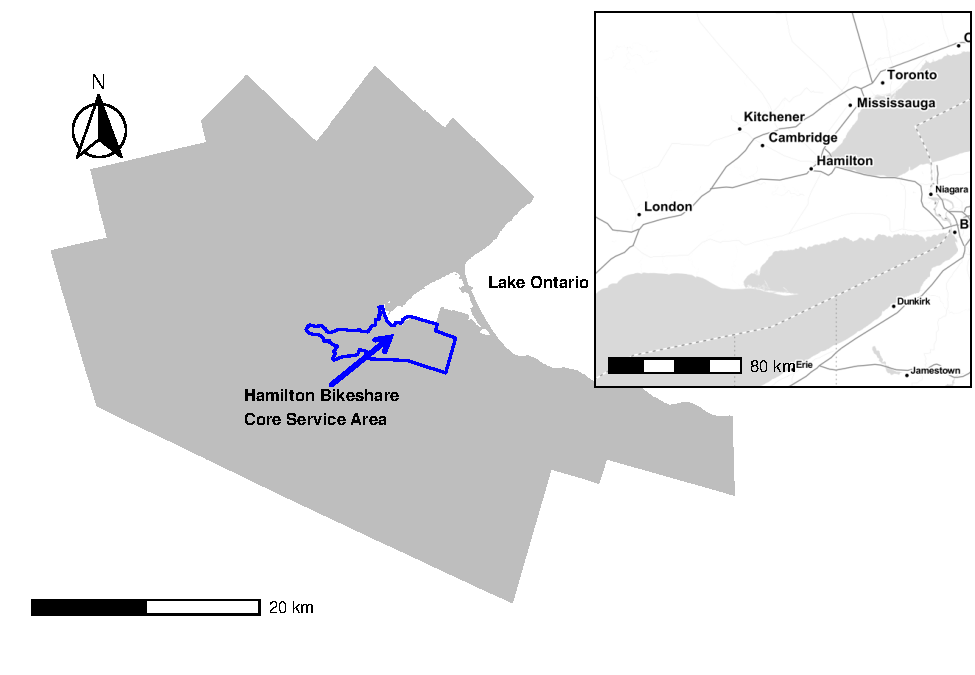
\includegraphics[width=0.65\linewidth]{Bike-share-spatial-equity_files/figure-latex/hamilton-and-sobi-service-area-1} 

}

\caption{The core service area of Hamilton Bike Share is outlined in black. Hamilton Census Metropolitan Area (CMA) is shown in grey.}\label{fig:hamilton-and-sobi-service-area}
\end{figure}

\begin{figure}

{\centering 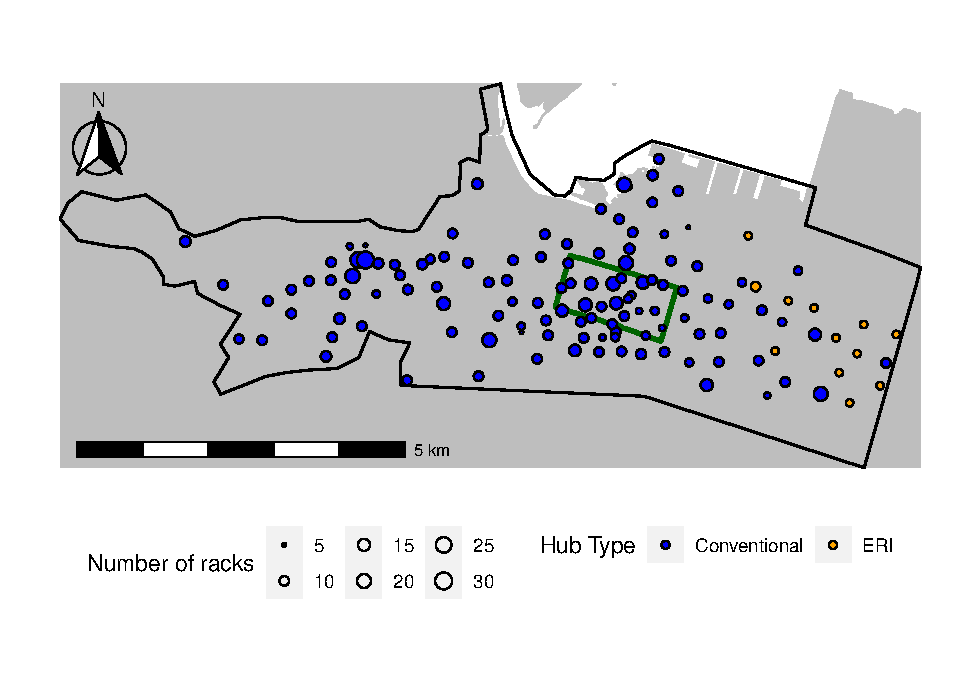
\includegraphics[width=1\linewidth]{Bike-share-spatial-equity_files/figure-latex/sobi-stations-in-hamilton-1} 

}

\caption{The spatial distribution of bike share stations in Hamilton, Ontario. The service area of Hamilton Bike Share is outlined in black and the city's downtown core is outlined in dark green. Hamilton CMA is shown in grey.}\label{fig:sobi-stations-in-hamilton}
\end{figure}

\hypertarget{sec:methods}{%
\section{Methods}\label{sec:methods}}

\hypertarget{floating-catchment-area}{%
\subsection{Floating Catchment Area}\label{floating-catchment-area}}

Floating catchment area (FCA) methods are an approach commonly used in
the healthcare accessibility literature. This approach is more
appropriate and informative than calculating the provider-to-population
ratio (PPR) which simply divides the level of supply of a service (e.g.,
the number of bicycle racks at a station) by the population who have
access to the service (Paez et al., 2019). In particular, the Two-Step
Floating Catchment Area method produces flexible catchment areas for
populations accessing a service rather than using rigid boundaries like
PPR, which provides more useful information because it takes into
account individual behaviour and doesn't assume that people stay within
the pre-defined boundaries (Paez et al., 2019). This is an important
property that supports our rationale for applying this method to measure
accessibility to Hamilton Bike Share. The City of Hamilton has
positioned stations between 300 and 600 metres apart, which would lead
to boundaries around these buffers, but it would be reasonable to assume
that people are willing to walk beyond this threshold to access other
stations if the ones nearest them have no supply of bicycles.

More recently, the \emph{balanced} floating catchment area approach was
developed to address issues with demand and supply inflation that are a
result of the overlapping catchment areas produced by the Two-Step
Floating Catchment Area (Paez et al., 2019). This overlap inflates the
demand and generates inaccurate or misleading accessibility estimates
(Paez et al., 2019). By adjusting the impedance weights, both supply and
demand are proportionally allocated which eliminates the double-counting
of population that leads to demand and supply inflation (Paez et al.,
2019). Other benefits of this adjusted method include consideration of
competition which can occur when catchment areas overlap, as well as the
preservation of system-wide population and level of service. Balanced
floating catchment area methods have been used to explore accessibility
to health care providers (Paez et al., 2019) and COVID-19 health care
services (Pereira et al., 2021), but have not yet been used in the
cycling literature to explore issues of accessibility.

In their review of accessibility measures, Geurs and van Wee (2004)
highlight the need for greater inclusion of individual spatio-temporal
constraints but acknowledge the challenges of acquiring and analyzing
person-based data. This comes after Kwan's (1998) work to show that
space-time measures are more capable of capturing interpersonal
differences, especially the effect of space-time constraints on
individual behaviour, and are more helpful for unraveling gender/ethnic
differences. Applying the balanced floating catchment area approach to
examine accessibility to Hamilton Bike Share constitutes a
location-based measure with an individual component by stratifying
according to median household income (Geurs and van Wee, 2004), but
conducting a further sensitivity analysis by adjusting distance
thresholds would introduce additional spatio-temporal constraints to
evaluate equitable accessibility.

The first step in the balanced floating catchment area method is to
allocate the population to be serviced by each Hamilton Bike Share
station: \[
P_j = {\sum_{i = 1}^{n} P_i{w_{ij}}}
\]

Next, the level of service at each station (i.e., the maximum number of
bicycle racks) is divided by its estimated service population within the
established catchment area: \[
L_j = \frac {S_j}{P_j} = \frac {S_j}{{\sum_{i = 1}^{n} P_i{w_{ij}}}}
\]

Finally, the accessibility of population cell \(i\) is calculated as the
weighted sum of the level of service of all stations that can be reached
from there according to normalized weights: \[
A_i = {\sum_{j = 1}^{J} L_j{w_{ji}}} = {\sum_{j = 1}^{J} \frac {S_j{w_{ji}}}{\sum_{i = 1}^{n} P_i{w_{ij}}}}
\]

The approach uses instead a set of suitably normalized weights as
follows: \[
{w_{ij}^{i} = \frac {w_{ij}}{\sum_{j = 1}^{J} {w_{ji}}}}
\]

and \[
{w_{ij}^{j} = \frac {w_{ij}}{\sum_{j = 1}^{J} {w_{ji}}}}
\]

These weights satisfy the following properties: \[
\sum_{j = 1}^{J} {w^i_{ji}} = 1
\]

and \[
\sum_{i = 1}^{n} {w^j_{ji}} = 1
\]

Finally, accessibility is calculated without risk of demand or supply
inflation: \[
A_i = {\sum_{j = 1}^{J} \frac {S_j{w^j_{ij}}}{\sum_{i = 1}^{n} P_i{w^i_{ij}}}}
\]

\hypertarget{pycnophylactic-interpolation}{%
\subsection{Pycnophylactic
Interpolation}\label{pycnophylactic-interpolation}}

Following the method first presented by Tobler (1979), we used
pycnophylactic interpolation to disaggregate population from each
dissemination area to smaller polygons that are 50 by 50 metres. This
method involves smoothing out the population from each dissemination
area while preserving total volume {[}see Figure
\ref{fig:da-population}{]}. Since pycnophylactic interpolation occurs at
such a micro scale, we had to ensure that population numbers were not
reallocated or smoothed out to areas where people do not live in
Hamilton (i.e., where schools or parks are located). To do so, we
retrieved shapefiles for various geographic features {[}see Table
\ref{tab:data-features}{]} from Open Hamilton. Next, we extracted these
features from the PBSP core service area and used pycnophylactic
interpolation to disaggregate and reallocate population {[}see Figure
\ref{fig:interpolated-population}{]}.

\begin{table}

\caption{\label{tab:data-features}\label{tab:landscape-features}Landscape features extracted from the Hamilton Bike Share core service area before population is interpolated.}
\centering
\resizebox{\linewidth}{!}{
\begin{tabular}[t]{>{}l|>{\raggedright\arraybackslash}p{30em}}
\toprule
Feature & Description\\
\midrule
\cellcolor{gray!6}{\textbf{Hamilton Bike Share Stations}} & \cellcolor{gray!6}{The location of stations and the number of racks available at each station.}\\
\textbf{Golf Courses} & The location of City and privately owned golf courses.\\
\cellcolor{gray!6}{\textbf{Parks}} & \cellcolor{gray!6}{The location of parks and other green spaces.}\\
\textbf{Designated Large Employment Areas} & The location of large business parks and industrial lands.\\
\cellcolor{gray!6}{\textbf{Municipal Parking Lots}} & \cellcolor{gray!6}{The location of municipal car parks.}\\
\addlinespace
\textbf{Cemeteries} & The location of cemeteries.\\
\cellcolor{gray!6}{\textbf{Environmentally Sensitive Areas}} & \cellcolor{gray!6}{The location of either land or water areas containing natural features or significant ecological functions.}\\
\textbf{Streets} & The street network in Hamilton, including road classification for highways.\\
\cellcolor{gray!6}{\textbf{Educational Institutions}} & \cellcolor{gray!6}{The location of all educational institutions and schools.}\\
\textbf{Places of Worship} & The location of buildings used for religious congregations.\\
\addlinespace
\cellcolor{gray!6}{\textbf{Municipal Service Centres}} & \cellcolor{gray!6}{The location of all municipal service centres, including City Hall.}\\
\textbf{Recreation and Community Centres} & The location of all recreation and community centres.\\
\cellcolor{gray!6}{\textbf{Arenas}} & \cellcolor{gray!6}{The location of all indoor arenas.}\\
\textbf{Emergency Stations} & The location of all Emergency Management Services (EMS) Ambulance stations.\\
\cellcolor{gray!6}{\textbf{Fire Stations}} & \cellcolor{gray!6}{The location of all fire stations.}\\
\addlinespace
\textbf{Police Stations} & The location of all police stations.\\
\cellcolor{gray!6}{\textbf{Railways}} & \cellcolor{gray!6}{The railway network in Hamilton.}\\
\textbf{Hospitals} & The location of all hospitals.\\
\bottomrule
\end{tabular}}
\end{table}

\begin{figure}

{\centering 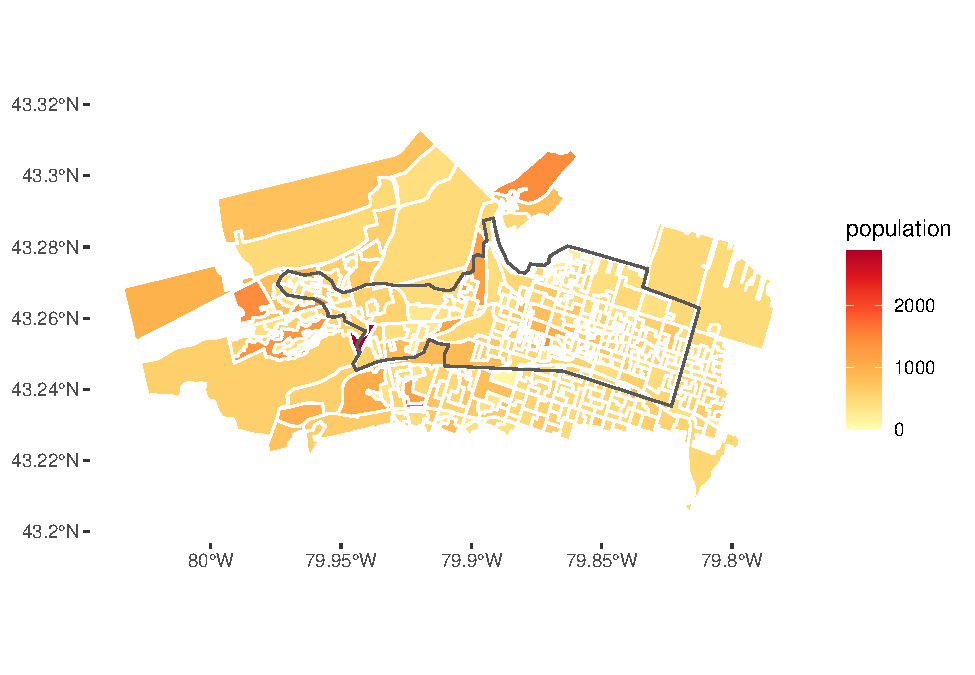
\includegraphics[width=0.65\linewidth]{Bike-share-spatial-equity_files/figure-latex/da-population-1} 

}

\caption{Population in all dissemination areas (outlined in white) in the Hamilton Bike Share core service area (outlined in black) and within 30 minutes of walking to the service area.}\label{fig:da-population}
\end{figure}

\begin{figure}

{\centering 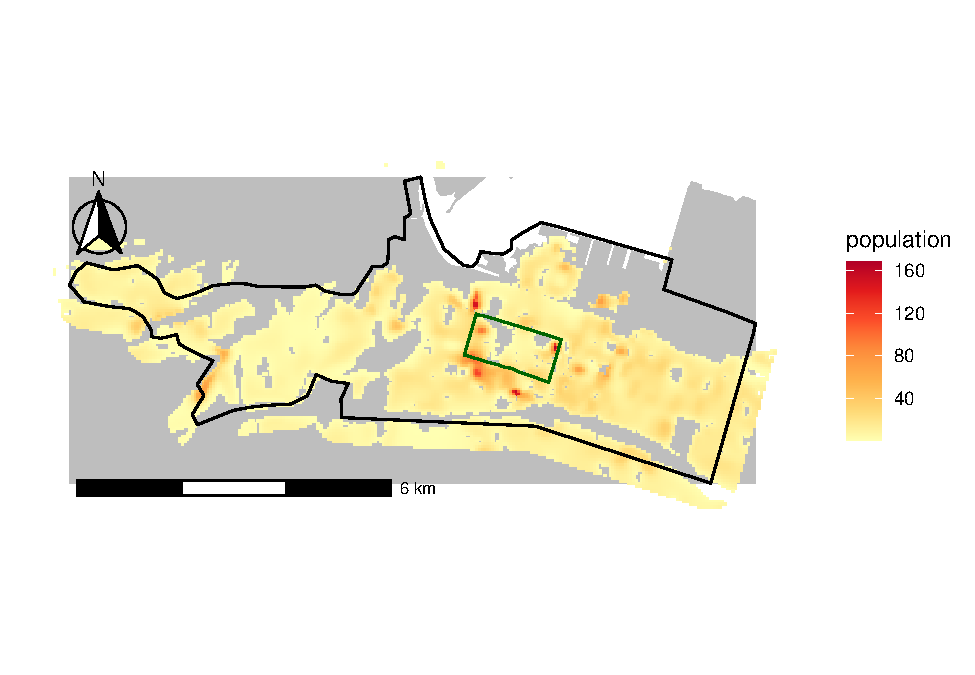
\includegraphics[width=0.65\linewidth]{Bike-share-spatial-equity_files/figure-latex/interpolated-population-1} 

}

\caption{Interpolated population in the Hamilton Bike Share core service area (outlined in black) and within 30 minutes of walking to the core service area (outlined in blue). The downtown area is outlined in dark green. Geographic features have been extracted. Dissemination area polygons are outlined in grey.}\label{fig:interpolated-population}
\end{figure}

\hypertarget{travel-time-matrix}{%
\subsection{Travel Time Matrix}\label{travel-time-matrix}}

\href{https://download.bbbike.org/osm/bbbike/}{BBBike} is an online
cycle route planner that interfaces with OpenStreetMap. We extracted
OpenStreetMap data for SoBi Hamilton's service area to calculate walking
times from each population cell to nearby bike share stations, using a
walking distance of 10km and a walking time of 30 minutes as a
threshold. A travel time matrix was created with the origins as the
coordinates of the population cells and the destinations as the
coordinates of the bike share stations within the maximum threshold.

\hypertarget{data}{%
\subsection{Data}\label{data}}

All data for this research were accessed from Open Hamilton\footnote{https://open.hamilton.ca/},
an online repository of data curated by the City of Hamilton.

\hypertarget{results}{%
\section{Results}\label{results}}

\hypertarget{accessibility-by-distance-thresholds}{%
\subsection{Accessibility by Distance
Thresholds}\label{accessibility-by-distance-thresholds}}

Consensus regarding the distance that individuals are willing to walk to
access a PBSP is lacking, therefore the literature on walking behaviour
was consulted to determine the thresholds for the sensitivity analysis.
Previous studies have found that living within 250 metres (Fuller et
al., 2011) and 300 metres (Kabra et al., 2020) is correlated with bike
share use, while other research has found that walking trips are less
than 600 metres and rarely more than 1200 metres (Millward et al., 2013)
or a median distance of 650 metres (Larsen et al., 2010). We found that
accessibility increases with a threshold between two and four minutes,
but is then maximized at 5 minutes. At some stations, Hamilton Bike
Share will depict a map to show the user the locations of the other
nearest stations within a five minute walk, which suggests that this is
an average distance that people are anticipated to walk. Accessibility
decreases significantly after eight minutes, which is intuitive given
that demand on a limited supply increases as more people can reach each
bike share station.

For this reason, we experiment with various walking thresholds by
conducting a sensitivity analysis to calculate accessibility at
different walking times: 3 minutes, 5 minutes, 10 minutes, and 15
minutes. We categorize these thresholds as minimum, average, maximum,
and extreme, respectively. At each threshold, we compare accessibility
between the current system and the original system to examine the
contribution of the additional equity stations.

\hypertarget{three-minutes}{%
\subsubsection{Three Minutes}\label{three-minutes}}

At the minimum threshold, we find that there are 25.2 bicycle racks per
person in the original system. With the addition of equity stations,
there are now 25.4 bicycles per person. Figure \ref{fig:figure-6}
presents a comparison of accessibility between the systems.
Accessibility is fairly uniform, with the exception of two small areas
near the university and the waterfront park where accessibility is
slightly higher.

\begin{figure}

{\centering 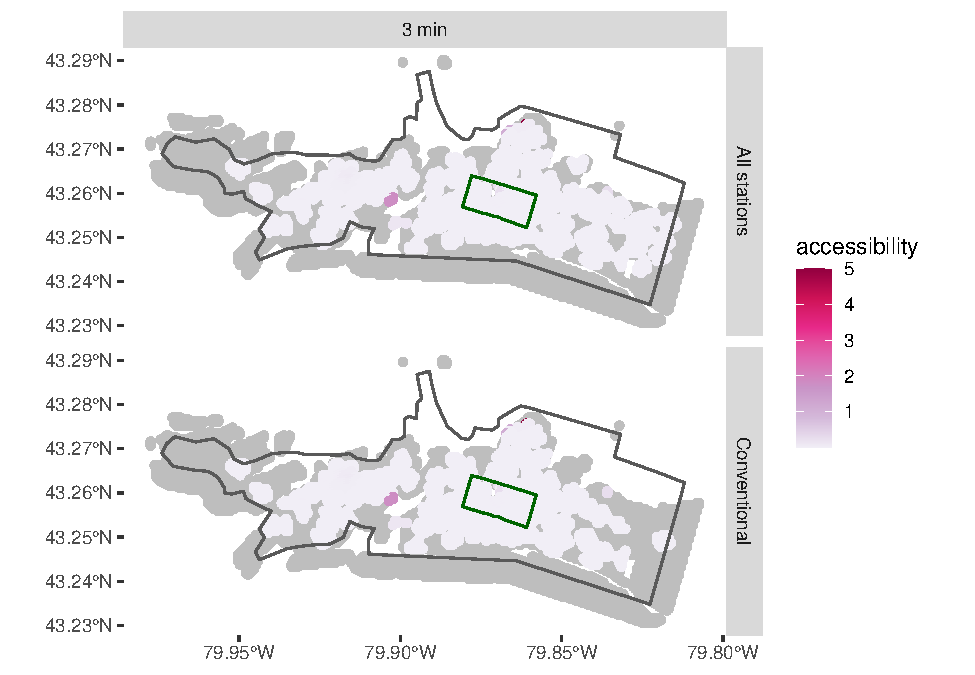
\includegraphics[width=0.65\linewidth]{Bike-share-spatial-equity_files/figure-latex/figure-6-1} 

}

\caption{Accessibility at 3 minutes walk (minimum threshold) compared between current system with equity stations and the original system without equity stations.}\label{fig:figure-6}
\end{figure}

\hypertarget{five-minutes}{%
\subsubsection{Five Minutes}\label{five-minutes}}

At the average threshold, we find that there are 68.6 bicycle racks per
person in the original system. With the addition of equity stations,
there are now 68.8 bicycles per person. Figure \ref{fig:figure-7}
presents a comparison of accessibility between the systems. Again,
accessibility is fairly uniform, with the exception of one very small
area near the waterfront park where accessibility is higher.

\begin{figure}

{\centering 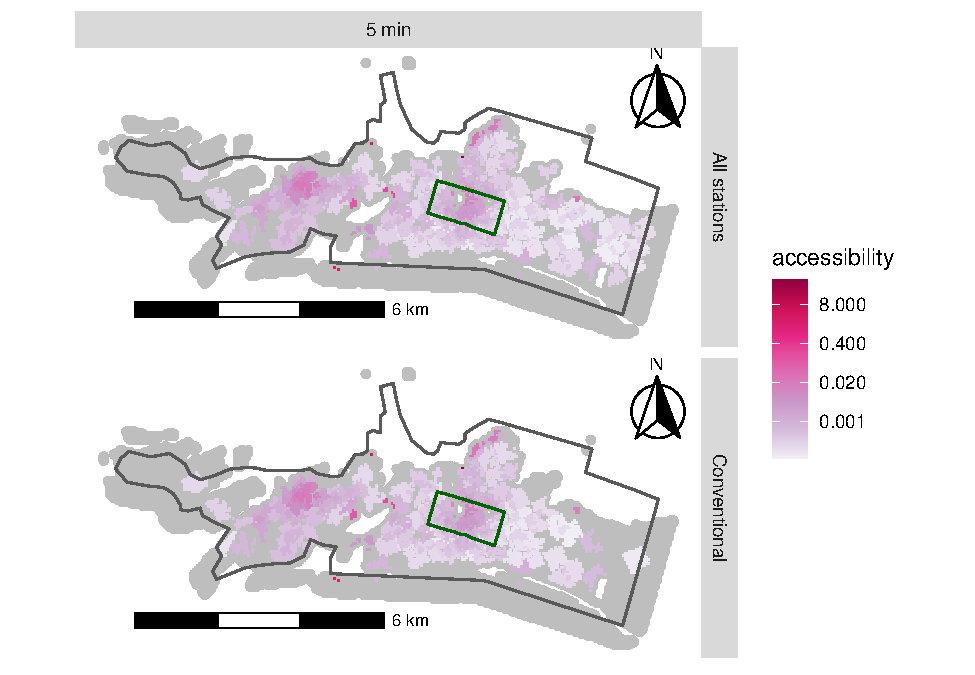
\includegraphics[width=0.65\linewidth]{Bike-share-spatial-equity_files/figure-latex/figure-7-1} 

}

\caption{Accessibility at 5 minutes walk (average threshold) compared between current system with equity stations and the original system without equity stations.}\label{fig:figure-7}
\end{figure}

\hypertarget{ten-minutes}{%
\subsubsection{Ten Minutes}\label{ten-minutes}}

At the maximum threshold, we find that there are 3.61 bicycle racks per
person in the original system. With the addition of equity stations,
there are now 3.74 bicycles per person. Figure \ref{fig:figure-8}
presents a comparison of accessibility between the systems. We begin to
see differences in accessibility across the service area, with users
near the university and its adjacent neighbourhoods, as well as
neighbourhoods north of the downtown area, have slightly higher
accessibility. While the differences are modest, they are more apparent
at this threshold than at shorter walking distances.

\begin{figure}

{\centering 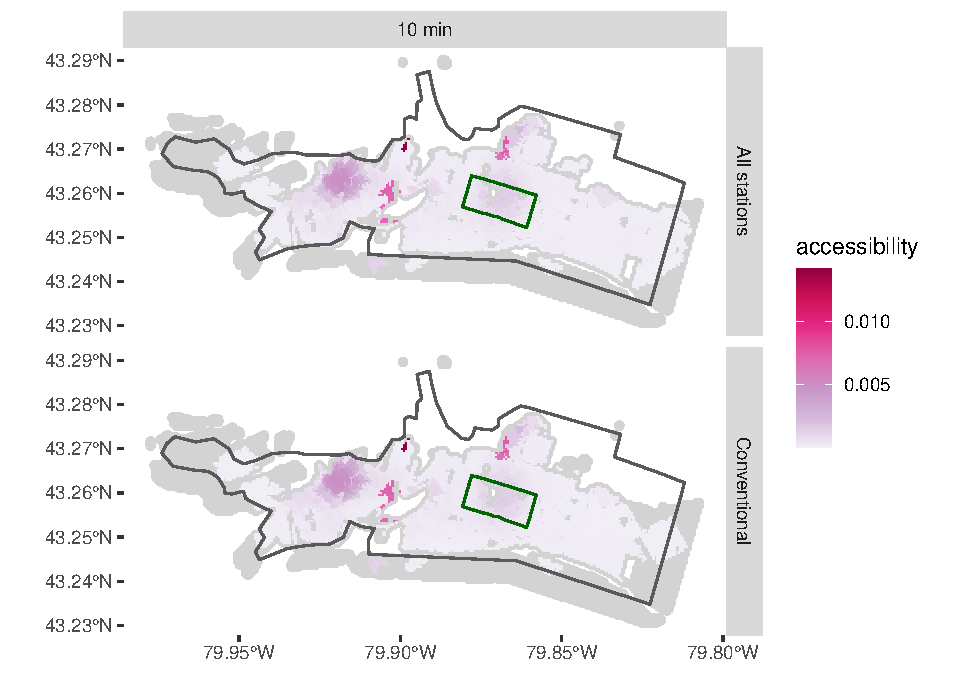
\includegraphics[width=0.65\linewidth]{Bike-share-spatial-equity_files/figure-latex/figure-8-1} 

}

\caption{Accessibility at 10 minutes walk (maximum threshold) compared between current system with equity stations and the original system without equity stations.}\label{fig:figure-8}
\end{figure}

\hypertarget{fifteen-minutes}{%
\subsubsection{Fifteen Minutes}\label{fifteen-minutes}}

At the extreme threshold, we find that there are 2.44 bicycle racks per
person in the original system. With the addition of equity stations,
there are now 2.55 bicycles per person. Figure \ref{fig:figure-9}
presents a comparison of accessibility between the systems. Users near
the university and the neighbourhoods north of the downtown area
(outlined in green) have the highest accessibility, followed by those
who live in the city's downtown area. Accessibility in the east end of
the core service area remains low.

\begin{figure}

{\centering 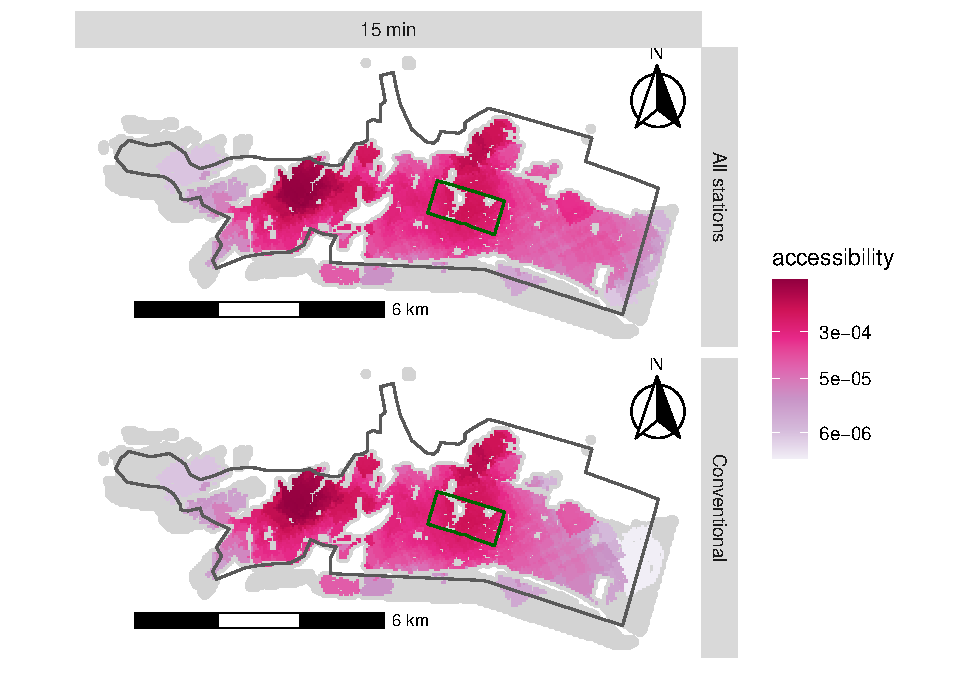
\includegraphics[width=0.65\linewidth]{Bike-share-spatial-equity_files/figure-latex/figure-9-1} 

}

\caption{Accessibility at 15 minutes walk (extreme threshold) compared between current system with equity stations and the original system without equity stations.}\label{fig:figure-9}
\end{figure}

\hypertarget{accessibility-by-median-total-income}{%
\subsection{Accessibility by Median Total
Income}\label{accessibility-by-median-total-income}}

Approximately 138,000 people live within Hamilton Bike Share's core
service area or within a 30 minute walk to the service area. We find
that over 118,000 people can access a bicycle share station within a 15
minute walk, which represents roughly 85\% of the total population in
the core service area {[}see Table \ref{tab:accessibility-income}{]}.
While previous research found that neighbourhoods with more disadvantage
are better serviced by Hamilton Bike Share (Hosford and Winters, 2018),
the authors used the Pampalon Deprivation Index from 2011 as a measure
of socioeconomic status for dissemination areas across the city not just
within the core service area. Instead, we use median total income for
each dissemination area in the core service area to examine whether
disparities in accessibility exist between income groups for those who
live in or near the core service area. We divide income by quantiles:
bottom 20\%, second 20\%, third 20\%, fourth 20\%, and top 20\%. One of
the unique properties of the balanced floating catchment area method is
that data can be reaggregated from small to larger polygons while
preserving the total population and supply at each station. This avoids
demand and supply inflation, and also enables us to present findings in
a way that is easier to interpret (i.e., across dissemination areas
instead of 50 by 50 metre population cells).

Panels 1{[}\ref{fig:figure-bi-map-threshold-3}{]}, 2
{[}\ref{fig:figure-bi-map-threshold-5}{]}, 3
{[}\ref{fig:figure-bi-map-threshold-10}{]}, and 4
{[}\ref{fig:figure-bi-map-threshold-15}{]} depict bivariate choropleth
maps with the combined spatial distribution of accessibility and median
total income per household for the different thresholds. Our analysis
demonstrates that the extreme threshold of fifteen minutes allows the
most people to access a station. We find that stations added to
Hamilton's public bicycle share program to increase equity for
disadvantaged neighbourhoods achieved their goal by increasing
accessibility, albeit only modestly {[}see Table
\ref{tab:accessibility-income}{]}. By implementing equity stations in
more areas with lower median total income in Hamilton, the PBSP has
achieved greater horizontal equity by extending the spatial distribution
of bicycles across the city. This is particularly evident at the minimum
and average thresholds of three and five minutes, respectively. The
largest gains were made for dissemination areas in the second 20\%,
where an additional 3,073 and 5,395 people could reach a bicycle share
station within three and five minutes walk, respectively, after the
addition of the equity station.

However, we found that dissemination areas with the lowest total
household income do not have much greater access to the program {[}see
Table \ref{tab:table-3}{]}. Income disparities still persist, however
only at certain thresholds. With and without equity stations, people in
the top 20\% of income have the highest level of accessibility at a
threshold of ten and fifteen minutes. Although dissemination areas in
the second 20\% have the highest level of accessibility by a significant
amount at lower thresholds, the bottom 20\%, who may benefit the most
from Hamilton Bike Share's equity initiatives, have the lowest
accessibility at three minutes threshold and the second lowest
accessibility at all other thresholds. Panels
1{[}\ref{fig:figure-bi-map-threshold-3}{]}, 2
{[}\ref{fig:figure-bi-map-threshold-5}{]}, 3
{[}\ref{fig:figure-bi-map-threshold-10}{]}, and 4
{[}\ref{fig:figure-bi-map-threshold-15}{]} reveal specific areas where
accessibility is low or zero, which are good candidates for additional
equity stations.

On the whole, we find that areas that have less than their equitable
share of the level of service are some of the most socioeconomically
disadvantaged areas in the city. While the addition of equity stations
increases accessibility for all income groups at all thresholds, they
did not increase accessibility significantly for any single income
group. This finding aligns with other studies that have found
disparities in station or bike location along income lines in New York
City (Babagoli et al., 2019), Tampa (Chen et al., 2019), and Seattle
(Mooney et al., 2019), where people who have greater advantage have
better access to PBSPs.

\begin{figure}
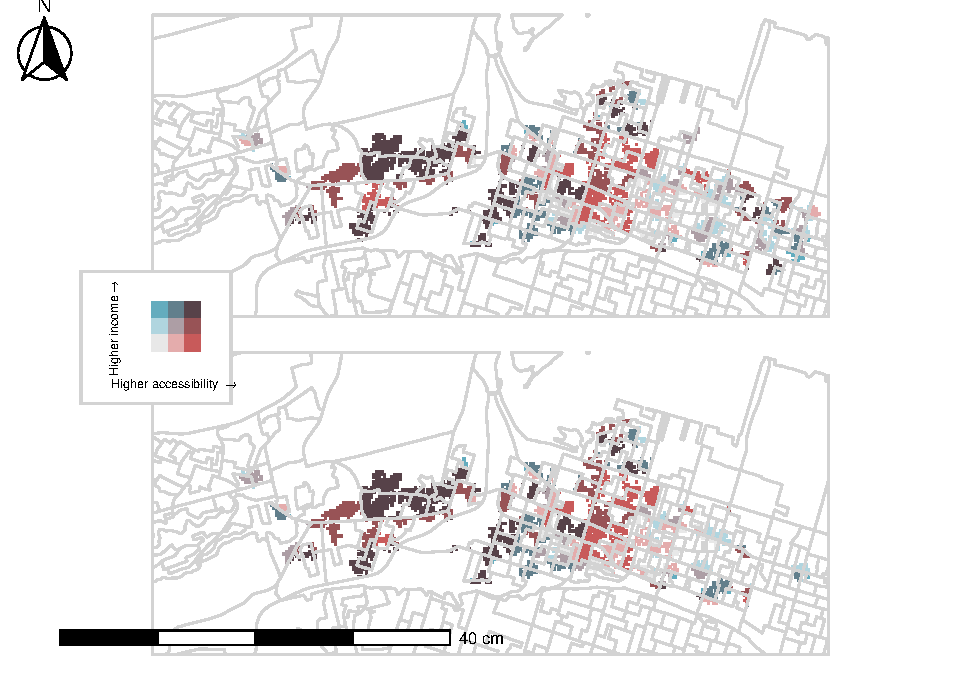
\includegraphics[width=1\linewidth]{Bike-share-spatial-equity_files/figure-latex/figure-bi-map-threshold-3-1} \caption{\label{fig-bivariate-map-threshold-3}Bivariate map of accessibility and income (threshold: 3 min): without equity stations (top panel) and with equity stations (bottom panel)}\label{fig:figure-bi-map-threshold-3}
\end{figure}

\begin{figure}
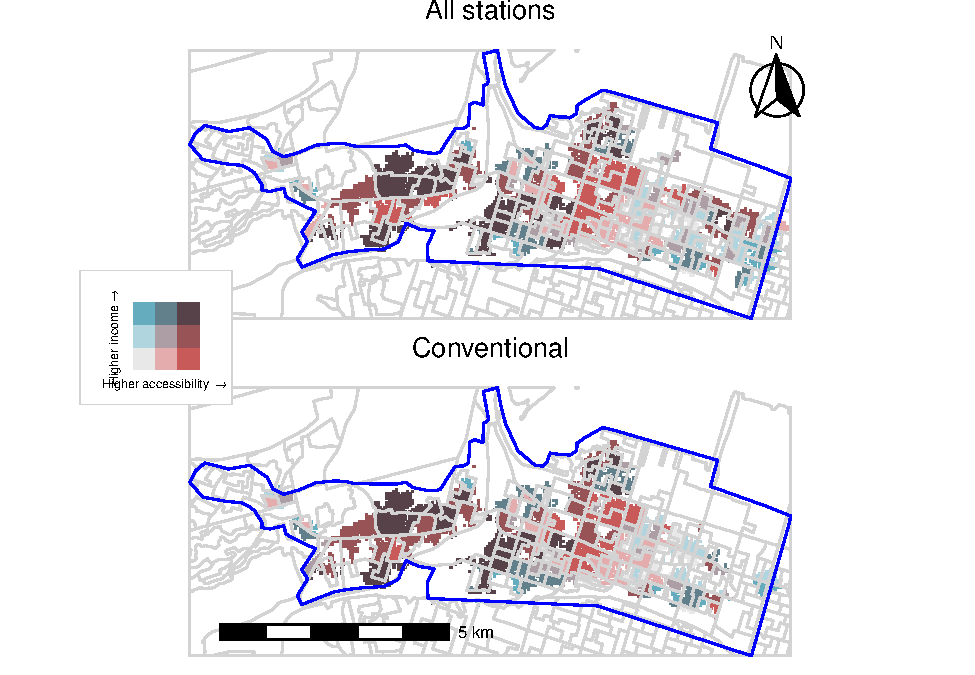
\includegraphics[width=1\linewidth]{Bike-share-spatial-equity_files/figure-latex/figure-bi-map-threshold-5-1} \caption{\label{fig-bivariate-map-threshold-5}Bivariate map of accessibility and income (threshold: 5 min): without equity stations (top panel) and with equity stations (bottom panel)}\label{fig:figure-bi-map-threshold-5}
\end{figure}

\begin{figure}
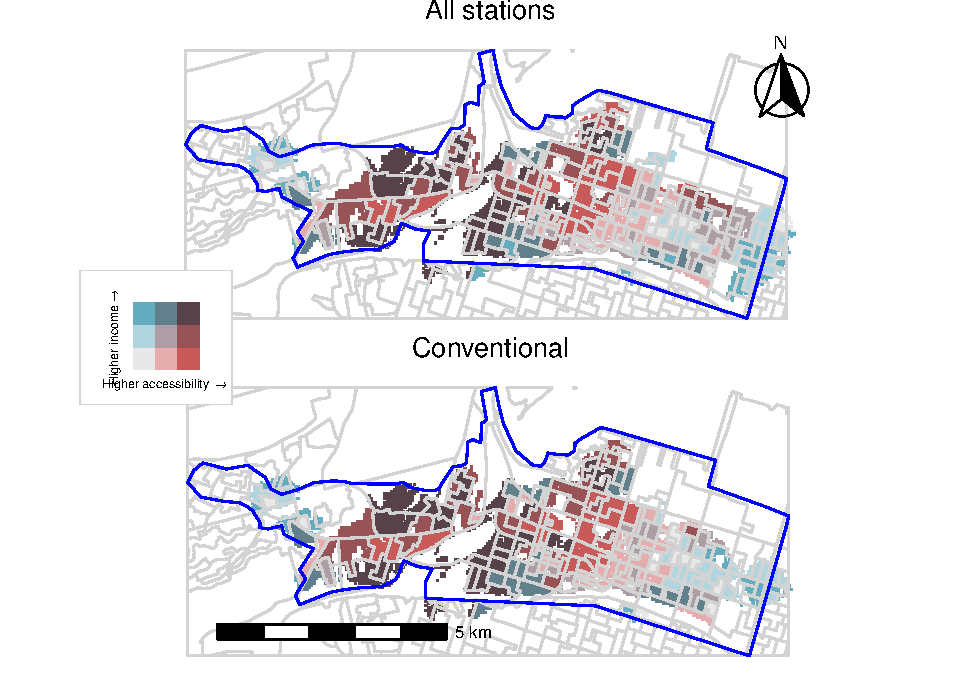
\includegraphics[width=1\linewidth]{Bike-share-spatial-equity_files/figure-latex/figure-bi-map-threshold-10-1} \caption{\label{fig-bivariate-map-threshold-10}Bivariate map of accessibility and income (threshold: 10 min): without equity stations (top panel) and with equity stations (bottom panel)}\label{fig:figure-bi-map-threshold-10}
\end{figure}

\begin{figure}
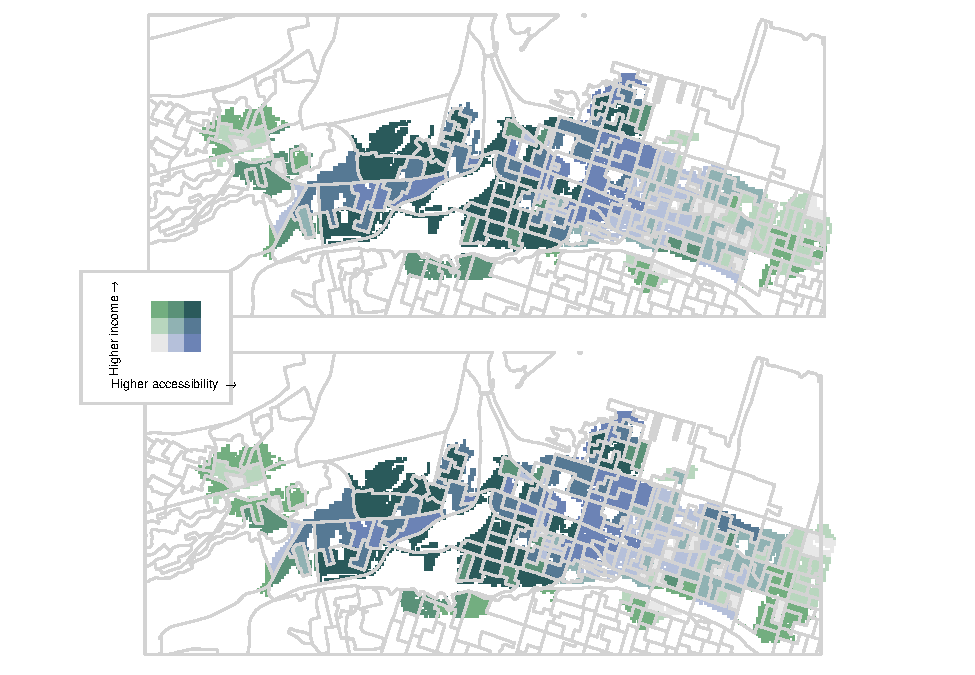
\includegraphics[width=1\linewidth]{Bike-share-spatial-equity_files/figure-latex/figure-bi-map-threshold-15-1} \caption{\label{fig-bivariate-map-threshold-15}Bivariate map of accessibility and income (threshold: 15 min): without equity stations (top panel) and equity stations (bottom panel)}\label{fig:figure-bi-map-threshold-15}
\end{figure}

\begin{table}

\caption{\label{tab:accessibility-income}\label{tab:accessibility-by-income}Accessibility and population serviced by income quintile and between systems (with and without equity stations).}
\centering
\resizebox{\linewidth}{!}{
\begin{tabular}[t]{lcccccc}
\toprule
\multicolumn{1}{c}{ } & \multicolumn{2}{c}{Without Equity Stations} & \multicolumn{2}{c}{With Equity Stations} & \multicolumn{2}{c}{Difference} \\
\cmidrule(l{3pt}r{3pt}){2-3} \cmidrule(l{3pt}r{3pt}){4-5} \cmidrule(l{3pt}r{3pt}){6-7}
Income Quintile & Accessibility & Population & Accessibility & Population & Accessibility & Population\\
\midrule
\addlinespace[0.3em]
\multicolumn{7}{l}{\textbf{Threshold - 3 minutes}}\\
\hspace{1em}\cellcolor{gray!6}{Bottom 20\%} & \cellcolor{gray!6}{2.377} & \cellcolor{gray!6}{22359} & \cellcolor{gray!6}{2.424} & \cellcolor{gray!6}{22798} & \cellcolor{gray!6}{0.047} & \cellcolor{gray!6}{439}\\
\hspace{1em}Second 20\% & 12.203 & 9347 & 12.281 & 12420 & 0.078 & 3073\\
\hspace{1em}\cellcolor{gray!6}{Third 20\%} & \cellcolor{gray!6}{3.093} & \cellcolor{gray!6}{7745} & \cellcolor{gray!6}{3.156} & \cellcolor{gray!6}{9455} & \cellcolor{gray!6}{0.063} & \cellcolor{gray!6}{1710}\\
\hspace{1em}Fourth 20\% & 4.119 & 1673 & 4.119 & 1673 & 0.000 & 0\\
\hspace{1em}\cellcolor{gray!6}{Top 20\%} & \cellcolor{gray!6}{3.408} & \cellcolor{gray!6}{2114} & \cellcolor{gray!6}{3.434} & \cellcolor{gray!6}{2379} & \cellcolor{gray!6}{0.026} & \cellcolor{gray!6}{265}\\
\addlinespace[0.3em]
\multicolumn{7}{l}{\textbf{Threshold - 5 minutes}}\\
\hspace{1em}Bottom 20\% & 1.302 & 35477 & 1.357 & 35803 & 0.055 & 326\\
\hspace{1em}\cellcolor{gray!6}{Second 20\%} & \cellcolor{gray!6}{56.048} & \cellcolor{gray!6}{17513} & \cellcolor{gray!6}{56.137} & \cellcolor{gray!6}{22908} & \cellcolor{gray!6}{0.089} & \cellcolor{gray!6}{5395}\\
\hspace{1em}Third 20\% & 4.258 & 15117 & 4.291 & 18309 & 0.033 & 3192\\
\hspace{1em}\cellcolor{gray!6}{Fourth 20\%} & \cellcolor{gray!6}{1.094} & \cellcolor{gray!6}{2867} & \cellcolor{gray!6}{1.095} & \cellcolor{gray!6}{3116} & \cellcolor{gray!6}{0.001} & \cellcolor{gray!6}{249}\\
\hspace{1em}Top 20\% & 5.925 & 4052 & 5.933 & 4518 & 0.008 & 466\\
\addlinespace[0.3em]
\multicolumn{7}{l}{\textbf{Threshold - 10 minutes}}\\
\hspace{1em}\cellcolor{gray!6}{Bottom 20\%} & \cellcolor{gray!6}{0.603} & \cellcolor{gray!6}{41824} & \cellcolor{gray!6}{0.621} & \cellcolor{gray!6}{41981} & \cellcolor{gray!6}{0.018} & \cellcolor{gray!6}{157}\\
\hspace{1em}Second 20\% & 0.860 & 27546 & 0.927 & 30503 & 0.067 & 2957\\
\hspace{1em}\cellcolor{gray!6}{Third 20\%} & \cellcolor{gray!6}{0.772} & \cellcolor{gray!6}{22394} & \cellcolor{gray!6}{0.799} & \cellcolor{gray!6}{25128} & \cellcolor{gray!6}{0.027} & \cellcolor{gray!6}{2734}\\
\hspace{1em}Fourth 20\% & 0.225 & 4544 & 0.227 & 4989 & 0.002 & 445\\
\hspace{1em}\cellcolor{gray!6}{Top 20\%} & \cellcolor{gray!6}{1.160} & \cellcolor{gray!6}{7989} & \cellcolor{gray!6}{1.162} & \cellcolor{gray!6}{9078} & \cellcolor{gray!6}{0.002} & \cellcolor{gray!6}{1089}\\
\addlinespace[0.3em]
\multicolumn{7}{l}{\textbf{Threshold - 15 minutes}}\\
\hspace{1em}Bottom 20\% & 0.534 & 42208 & 0.554 & 42327 & 0.020 & 119\\
\hspace{1em}\cellcolor{gray!6}{Second 20\%} & \cellcolor{gray!6}{0.551} & \cellcolor{gray!6}{30507} & \cellcolor{gray!6}{0.611} & \cellcolor{gray!6}{31069} & \cellcolor{gray!6}{0.060} & \cellcolor{gray!6}{562}\\
\hspace{1em}Third 20\% & 0.546 & 26108 & 0.573 & 26660 & 0.027 & 552\\
\hspace{1em}\cellcolor{gray!6}{Fourth 20\%} & \cellcolor{gray!6}{0.093} & \cellcolor{gray!6}{6312} & \cellcolor{gray!6}{0.096} & \cellcolor{gray!6}{7435} & \cellcolor{gray!6}{0.003} & \cellcolor{gray!6}{1123}\\
\hspace{1em}Top 20\% & 0.712 & 10209 & 0.714 & 11089 & 0.002 & 880\\
\bottomrule
\multicolumn{7}{l}{\rule{0pt}{1em}\textit{Note: }}\\
\multicolumn{7}{l}{\rule{0pt}{1em} }\\
\multicolumn{7}{l}{\rule{0pt}{1em}\textsuperscript{a} With equity stations = Hamilton Bike Share current system (118 conventional stations, 12 equity stations)}\\
\multicolumn{7}{l}{\rule{0pt}{1em}\textsuperscript{b} Without equity stations = Hamilton Bike Share original system (118 conventional stations, no equity stations)}\\
\end{tabular}}
\end{table}

\hypertarget{study-limitations}{%
\section{Study Limitations}\label{study-limitations}}

This paper did not examine or compare ridership data between
conventional and equity stations. Therefore, further research is needed
to determine whether the addition of equity stations encouraged more
cycling for low-income individuals living near them. Other studies have
specifically looked at differences in trip type, frequency, or length
among users from disadvantaged neighbourhoods (Caspi and Noland, 2019;
Qian and Jaller, 2020; J. Wang and Lindsey, 2019a), but our analysis is
limited by the lack of accessible route or user data to conduct similar
analyses for Hamilton Bike Share.

\hypertarget{conclusion}{%
\section{Conclusion}\label{conclusion}}

The addition of specific equity stations to the public bicycle share
program in Hamilton, Ontario had the net effect of increasing
accessibility and reducing both horizontal and vertical inequities. In
particular, accessibility improved the most for the second 20\% median
total income groups at all thresholds, but the gains were only modest
for all income groups. Dissemination areas with the bottom 20\% had the
lowest accessibility at three minutes, and second lowest level of
accessibility at five, ten, and fifteen minutes. Congestion effects were
observed at higher thresholds, with accessibility decreasing
significantly once the catchment area is increased to 10 minutes
walking. Based on our analysis, we identified specific areas that have
both low accessibility and low income which would benefit from an
increased supply of bicycles. These are ideal candidates for new equity
stations. In this way, our paper has made contributions in a positive
way by applying an intuitive and useful approach to measure
accessibility to a PBSP, and in a normative way by serving to inform
future investments in cycle infrastructure for Hamilton Bike Share.

Wang and Lindsey (2019b) have noted that there is a lack of research
that examines how bike share users' behaviour changes as a result of
program changes to station locations or improvements in accessibility.
As such, a logical next step to this research is to examine whether
Hamilton Bike Share's equity stations increased ridership or resulted in
new memberships in areas that were previously under-served. An
examination of the types of trips undertaken by residents in these areas
would also be informative, such as the study undertaken by Caspi and
Norland (2019) after bike share stations were implemented in low-income
Philadelphia neighbourhoods. The bulk of cycling facilities that have
been built in Hamilton to date located in the core service area near the
conventional stations. It would be worthwhile to explore the route
choice of bike share trips departing or ending at the equity stations
and to identify factors that specifically influence trips from these
stations, which would extend existing studies conducted by Scott and
colleagues (Lu et al., 2018; Scott and Ciuro, 2019; Scott et al., 2021).
This paper, combined with additional studies such as those
conceptualized above, would serve as a valuable case study for Hamilton
and other cities with PBSPs who wish to evaluate and address spatial
inequities in accessibility and transportation options in urban areas.

\hypertarget{references}{%
\section*{References}\label{references}}
\addcontentsline{toc}{section}{References}

\hypertarget{refs}{}
\leavevmode\hypertarget{ref-auchinclossDesignBaselineDescription2020}{}%
Auchincloss, A.H., Michael, Y.L., Fuller, D., Li, S., Niamatullah, S.,
Fillmore, C.E., Setubal, C., Bettigole, C., 2020. Design and baseline
description of a cohort of bikeshare users in the city of Philadelphia.
Journal of Transport \& Health 16, 100836.
doi:\href{https://doi.org/10.1016/j.jth.2020.100836}{10.1016/j.jth.2020.100836}

\leavevmode\hypertarget{ref-babagoliExploringHealthSpatial2019}{}%
Babagoli, M.A., Kaufman, T.K., Noyes, P., Sheffield, P.E., 2019.
Exploring the health and spatial equity implications of the New York
City Bike share system. Journal of Transport \& Health 13, 200--209.
doi:\href{https://doi.org/10.1016/j.jth.2019.04.003}{10.1016/j.jth.2019.04.003}

\leavevmode\hypertarget{ref-breyWantRideMy2017}{}%
Brey, R., Castillo-Manzano, J.I., Castro-Nuño, M., 2017. ``I want to
ride my bicycle'': Delimiting cyclist typologies. Applied Economics
Letters 24, 549--552.
doi:\href{https://doi.org/10.1080/13504851.2016.1210760}{10.1080/13504851.2016.1210760}

\leavevmode\hypertarget{ref-buckAreBikeshareUsers2013}{}%
Buck, D., Buehler, R., Happ, P., Rawls, B., Chung, P., Borecki, N.,
2013. Are Bikeshare Users Different from Regular Cyclists?: A First Look
at Short-Term Users, Annual Members, and Area Cyclists in the
Washington, D.C., Region. Transportation Research Record 2387, 112--119.
doi:\href{https://doi.org/10.3141/2387-13}{10.3141/2387-13}

\leavevmode\hypertarget{ref-caspiBikesharingPhiladelphiaLowerincome2019}{}%
Caspi, O., Noland, R.B., 2019. Bikesharing in Philadelphia: Do
lower-income areas generate trips? Travel Behaviour and Society 16,
143--152.
doi:\href{https://doi.org/10.1016/j.tbs.2019.05.004}{10.1016/j.tbs.2019.05.004}

\leavevmode\hypertarget{ref-chenExploringEquityPerformance2019}{}%
Chen, Z., Guo, Y., Stuart, A.L., Zhang, Y., Li, X., 2019. Exploring the
equity performance of bike-sharing systems with disaggregated data: A
story of southern Tampa. Transportation Research Part A: Policy and
Practice 130, 529--545.
doi:\href{https://doi.org/10.1016/j.tra.2019.09.048}{10.1016/j.tra.2019.09.048}

\leavevmode\hypertarget{ref-chenUnobservedHeterogeneityTransportation2021}{}%
Chen, Z., Li, X., 2021. Unobserved heterogeneity in transportation
equity analysis: Evidence from a bike-sharing system in southern Tampa.
Journal of Transport Geography 91, 102956.
doi:\href{https://doi.org/10.1016/j.jtrangeo.2021.102956}{10.1016/j.jtrangeo.2021.102956}

\leavevmode\hypertarget{ref-civicplanSoBiHamiltonMembership2017}{}%
Civicplan, 2017. SoBi Hamilton Membership Survey. Civicplan \textbar{}
Planning Engagement Research.

\leavevmode\hypertarget{ref-fishmanBikeshareReviewRecent2016}{}%
Fishman, E., 2016. Bikeshare: A Review of Recent Literature. Transport
Reviews 36, 92--113.
doi:\href{https://doi.org/10.1080/01441647.2015.1033036}{10.1080/01441647.2015.1033036}

\leavevmode\hypertarget{ref-fishmanBarriersBikesharingAnalysis2014}{}%
Fishman, E., Washington, S., Haworth, N., Mazzei, A., 2014. Barriers to
bikesharing: An analysis from Melbourne and Brisbane. Journal of
Transport Geography 41, 325--337.
doi:\href{https://doi.org/10.1016/j.jtrangeo.2014.08.005}{10.1016/j.jtrangeo.2014.08.005}

\leavevmode\hypertarget{ref-fullerUseNewPublic2011}{}%
Fuller, D., Gauvin, L., Kestens, Y., Daniel, M., Fournier, M., Morency,
P., Drouin, L., 2011. Use of a New Public Bicycle Share Program in
Montreal, Canada. American Journal of Preventive Medicine 41, 80--83.
doi:\href{https://doi.org/10.1016/j.amepre.2011.03.002}{10.1016/j.amepre.2011.03.002}

\leavevmode\hypertarget{ref-geursAccessibilityEvaluationLanduse2004}{}%
Geurs, K.T., van Wee, B., 2004. Accessibility evaluation of land-use and
transport strategies: Review and research directions. Journal of
Transport Geography 12, 127--140.
doi:\href{https://doi.org/10.1016/j.jtrangeo.2003.10.005}{10.1016/j.jtrangeo.2003.10.005}

\leavevmode\hypertarget{ref-hamiltonHamiltonBikeShare2015}{}%
Hamilton, C. of, 2015. Hamilton Bike Share.

\leavevmode\hypertarget{ref-handyMeasuringAccessibilityExploration1997}{}%
Handy, S.L., Niemeier, D.A., 1997. Measuring Accessibility: An
Exploration of Issues and Alternatives. Environment and Planning A:
Economy and Space 29, 1175--1194.
doi:\href{https://doi.org/10.1068/a291175}{10.1068/a291175}

\leavevmode\hypertarget{ref-hosfordEvaluationImpactPublic2018}{}%
Hosford, K., Fuller, D., Lear, S.A., Teschke, K., Gauvin, L., Brauer,
M., Winters, M., 2018. Evaluation of the impact of a public bicycle
share program on population bicycling in Vancouver, BC. Preventive
Medicine Reports 12, 176--181.
doi:\href{https://doi.org/10.1016/j.pmedr.2018.09.014}{10.1016/j.pmedr.2018.09.014}

\leavevmode\hypertarget{ref-hosfordWhoArePublic2018}{}%
Hosford, K., Winters, M., 2018. Who Are Public Bicycle Share Programs
Serving? An Evaluation of the Equity of Spatial Access to Bicycle Share
Service Areas in Canadian Cities. Transportation Research Record 2672,
42--50.
doi:\href{https://doi.org/10.1177/0361198118783107}{10.1177/0361198118783107}

\leavevmode\hypertarget{ref-hosfordEvaluatingImpactImplementing2019}{}%
Hosford, K., Winters, M., Gauvin, L., Camden, A., Dubé, A.-S., Friedman,
S.M., Fuller, D., 2019. Evaluating the impact of implementing public
bicycle share programs on cycling: The International Bikeshare Impacts
on Cycling and Collisions Study (IBICCS). International Journal of
Behavioral Nutrition and Physical Activity 16, 107.
doi:\href{https://doi.org/10.1186/s12966-019-0871-9}{10.1186/s12966-019-0871-9}

\leavevmode\hypertarget{ref-hullgrassoBikeShareEquity2020}{}%
Hull Grasso, S., Barnes, P., Chavis, C., 2020. Bike Share Equity for
Underrepresented Groups: Analyzing Barriers to System Usage in
Baltimore, Maryland. Sustainability 12, 7600.
doi:\href{https://doi.org/10.3390/su12187600}{10.3390/su12187600}

\leavevmode\hypertarget{ref-kabraBikeShareSystemsAccessibility2020}{}%
Kabra, A., Belavina, E., Girotra, K., 2020. Bike-Share Systems:
Accessibility and Availability. Management Science 66, 3803--3824.
doi:\href{https://doi.org/10.1287/mnsc.2019.3407}{10.1287/mnsc.2019.3407}

\leavevmode\hypertarget{ref-kwanSpaceTimeIntegral1998}{}%
Kwan, M.-P., 1998. Space-Time and Integral Measures of Individual
Accessibility: A Comparative Analysis Using a Point-based Framework.
Geographical Analysis 30, 191--216.
doi:\href{https://doi.org/10.1111/j.1538-4632.1998.tb00396.x}{10.1111/j.1538-4632.1998.tb00396.x}

\leavevmode\hypertarget{ref-larsenQuarterMileReexamining2010}{}%
Larsen, J., El-Geneidy, A., Yasmin, F., 2010. Beyond the Quarter Mile:
Re-examining Travel Distances by Active Transportation. Canadian Journal
of Urban Research 19, 70--88.

\leavevmode\hypertarget{ref-levineCenturyEvolutionAccessibility2020}{}%
Levine, J., 2020. A century of evolution of the accessibility concept.
Transportation Research Part D: Transport and Environment 83, 102309.
doi:\href{https://doi.org/10.1016/j.trd.2020.102309}{10.1016/j.trd.2020.102309}

\leavevmode\hypertarget{ref-luUnderstandingBikeShare2018}{}%
Lu, W., Scott, D.M., Dalumpines, R., 2018. Understanding bike share
cyclist route choice using GPS data: Comparing dominant routes and
shortest paths. Journal of Transport Geography 71, 172--181.
doi:\href{https://doi.org/10.1016/j.jtrangeo.2018.07.012}{10.1016/j.jtrangeo.2018.07.012}

\leavevmode\hypertarget{ref-macarthurAdaptiveBikeShare2020}{}%
MacArthur, J., McNeil, N., Cummings, A., Broach, J., 2020. Adaptive Bike
Share: Expanding Bike Share to People with Disabilities and Older
Adults. Transportation Research Record 2674, 556--565.
doi:\href{https://doi.org/10.1177/0361198120925079}{10.1177/0361198120925079}

\leavevmode\hypertarget{ref-millwardActivetransportWalkingBehavior2013}{}%
Millward, H., Spinney, J., Scott, D., 2013. Active-transport walking
behavior: Destinations, durations, distances. Journal of Transport
Geography 28, 101--110.
doi:\href{https://doi.org/10.1016/j.jtrangeo.2012.11.012}{10.1016/j.jtrangeo.2012.11.012}

\leavevmode\hypertarget{ref-mooneyFreedomStationSpatial2019}{}%
Mooney, S.J., Hosford, K., Howe, B., Yan, A., Winters, M., Bassok, A.,
Hirsch, J.A., 2019. Freedom from the station: Spatial equity in access
to dockless bike share. Journal of Transport Geography 74, 91--96.
doi:\href{https://doi.org/10.1016/j.jtrangeo.2018.11.009}{10.1016/j.jtrangeo.2018.11.009}

\leavevmode\hypertarget{ref-nickkarSpatialtemporalGenderLand2019}{}%
Nickkar, A., Banerjee, S., Chavis, C., Bhuyan, I.A., Barnes, P., 2019. A
spatial-temporal gender and land use analysis of bikeshare ridership:
The case study of Baltimore City. City, Culture and Society 18, 100291.
doi:\href{https://doi.org/10.1016/j.ccs.2019.100291}{10.1016/j.ccs.2019.100291}

\leavevmode\hypertarget{ref-paezDemandLevelService2019}{}%
Paez, A., Higgins, C.D., Vivona, S.F., 2019. Demand and level of service
inflation in Floating Catchment Area (FCA) methods. PLoS ONE 14.
doi:\href{https://doi.org/10.1371/journal.pone.0218773}{10.1371/journal.pone.0218773}

\leavevmode\hypertarget{ref-paezMeasuringAccessibilityPositive2012}{}%
Páez, A., Scott, D.M., Morency, C., 2012. Measuring accessibility:
Positive and normative implementations of various accessibility
indicators. Journal of Transport Geography, Special Section on
Accessibility and Socio-Economic Activities: Methodological and
Empirical Aspects 25, 141--153.
doi:\href{https://doi.org/10.1016/j.jtrangeo.2012.03.016}{10.1016/j.jtrangeo.2012.03.016}

\leavevmode\hypertarget{ref-pereiraGeographicAccessCOVID192021}{}%
Pereira, R.H.M., Braga, C.K.V., Servo, L.M., Serra, B., Amaral, P.,
Gouveia, N., Paez, A., 2021. Geographic access to COVID-19 healthcare in
Brazil using a balanced float catchment area approach. Social Science \&
Medicine 273, 113773.
doi:\href{https://doi.org/10.1016/j.socscimed.2021.113773}{10.1016/j.socscimed.2021.113773}

\leavevmode\hypertarget{ref-qianBikesharingEquityDisadvantaged2020}{}%
Qian, X., Jaller, M., 2020. Bikesharing, equity, and disadvantaged
communities: A case study in Chicago. Transportation Research Part A:
Policy and Practice 140, 354--371.
doi:\href{https://doi.org/10.1016/j.tra.2020.07.004}{10.1016/j.tra.2020.07.004}

\leavevmode\hypertarget{ref-reillyNoncyclistsFrequentCyclists2020}{}%
Reilly, K.H., Noyes, P., Crossa, A., 2020. From non-cyclists to frequent
cyclists: Factors associated with frequent bike share use in New York
City. Journal of Transport \& Health 16, 100790.
doi:\href{https://doi.org/10.1016/j.jth.2019.100790}{10.1016/j.jth.2019.100790}

\leavevmode\hypertarget{ref-reillyGenderDisparitiesNew2020}{}%
Reilly, K.H., Wang, S.M., Crossa, A., 2020. Gender disparities in New
York City bike share usage. International Journal of Sustainable
Transportation 0, 1--9.
doi:\href{https://doi.org/10.1080/15568318.2020.1861393}{10.1080/15568318.2020.1861393}

\leavevmode\hypertarget{ref-scottWhatFactorsInfluence2019}{}%
Scott, D.M., Ciuro, C., 2019. What factors influence bike share
ridership? An investigation of Hamilton, Ontario's bike share hubs.
Travel Behaviour and Society 16, 50--58.
doi:\href{https://doi.org/10.1016/j.tbs.2019.04.003}{10.1016/j.tbs.2019.04.003}

\leavevmode\hypertarget{ref-scottRouteChoiceBike2021}{}%
Scott, D.M., Lu, W., Brown, M.J., 2021. Route choice of bike share
users: Leveraging GPS data to derive choice sets. Journal of Transport
Geography 90, 102903.
doi:\href{https://doi.org/10.1016/j.jtrangeo.2020.102903}{10.1016/j.jtrangeo.2020.102903}

\leavevmode\hypertarget{ref-toblerSmoothPycnophylacticInterpolation1979}{}%
Tobler, W.R., 1979. Smooth Pycnophylactic Interpolation for Geographical
Regions. Journal of the American Statistical Association 74, 519--530.
doi:\href{https://doi.org/10.1080/01621459.1979.10481647}{10.1080/01621459.1979.10481647}

\leavevmode\hypertarget{ref-wangNeighborhoodSociodemographicCharacteristics2019}{}%
Wang, J., Lindsey, G., 2019a. Neighborhood socio-demographic
characteristics and bike share member patterns of use. Journal of
Transport Geography 79, 102475.
doi:\href{https://doi.org/10.1016/j.jtrangeo.2019.102475}{10.1016/j.jtrangeo.2019.102475}

\leavevmode\hypertarget{ref-wangNewBikeShare2019}{}%
Wang, J., Lindsey, G., 2019b. Do new bike share stations increase member
use: A quasi-experimental study. Transportation Research Part A: Policy
and Practice 121, 1--11.
doi:\href{https://doi.org/10.1016/j.tra.2019.01.004}{10.1016/j.tra.2019.01.004}

\leavevmode\hypertarget{ref-wintersWhoAreSuperusers2019}{}%
Winters, M., Hosford, K., Javaheri, S., 2019. Who are the
``super-users'' of public bike share? An analysis of public bike share
members in Vancouver, BC. Preventive Medicine Reports 15, 100946.
doi:\href{https://doi.org/10.1016/j.pmedr.2019.100946}{10.1016/j.pmedr.2019.100946}


\end{document}


